\documentclass[12pt]{article}

\usepackage[utf8]{inputenc}
\usepackage[T1]{fontenc}
\usepackage{amsmath,amssymb}
\usepackage{graphicx}
\usepackage{caption}
\usepackage{helvet}
\usepackage{hyperref}
\usepackage{bookmark}
\usepackage{framed}
\usepackage{listings}
\usepackage{mdframed}
\usepackage{sectsty}
\usepackage{tikz}
\usepackage{geometry}
\geometry{a4paper,margin=2.5cm}


\graphicspath{{img/}}

\newcommand{\abs}[1]{\left|#1\right|}

\sectionfont{\fontsize{10}{12}\selectfont}
\subsectionfont{\fontsize{10}{12}\selectfont}
\subsubsectionfont{\fontsize{10}{12}\selectfont}

\lstset{
  language=Matlab,
  basicstyle=\ttfamily\footnotesize,
  keywordstyle=\color{blue},
  commentstyle=\color{green!50!black},
  stringstyle=\color{red!60!black},
  frame=single,
  breaklines=true,
  keepspaces=true,
  showspaces=false,
  showstringspaces=false
}

\begin{document}

% ===================== TITOLO =====================
\begin{titlepage}
  \centering
  {\Huge \textbf{Università degli Studi di Padova}\par}
  \vspace{1cm}
  \begin{figure}[htbp!]
    \centering
    
\includegraphics[width=0.45\textwidth]{logo_unipd.png}
  \end{figure}
  \vspace{1.5cm}
  {\LARGE \textbf{Relazione per:}\par}
  {\Huge \textbf{INTERPOLAZIONE POLINOMIALE CON NODI DI LEJA\\APPROSSIMATI}\par}
  \vfill
  \textbf{Realizzata da:}\par
  Oliver Florin Stiglet, matricola 2044895\par
  \vspace{0.5cm}
  \textbf{Corso:} Programmazione/Calcolo Numerico (MATLAB)\par
  \vspace{0.2cm}
  \textbf{Data:} \today
\end{titlepage}

\renewcommand{\familydefault}{\sfdefault}
\fontsize{10}{12}\selectfont

% ===================== INTRO =====================
\section{Introduzione}
Obiettivo del progetto: implementare in \textsc{Matlab} l'interpolazione polinomiale su \([{-}1,1]\) utilizzando \emph{punti di Leja approssimati} estratti da una mesh fitta, calcolare la \emph{costante di Lebesgue} per valutarne la stabilità, e confrontare l'accuratezza dell'interpolante con quella ottenuta usando \emph{nodi equispaziati}.\\[2mm]
Sia \(\{z_i\}_{i=0}^d\) l'insieme dei nodi. L'interpolante è costruito su base di \textbf{Chebyshev} di primo tipo:
\[
V_{ij}=\cos\!\big((j{-}1)\arccos(z_i)\big),\qquad i=1,\dots,d{+}1,\ j=1,\dots,d{+}1,
\]
e i coefficienti si ottengono risolvendo il sistema lineare \(V\,c=f(z)\) con l'operatore \verb|\| di MATLAB, senza usare \verb|polyfit|.

% ===================== ALGORITMI =====================
\section{Algoritmi implementati}

\subsection{Algoritmo 1: DLP (produttoria)}
A partire dal primo nodo \(z_0=x(1)\) (primo elemento della mesh), il nodo successivo massimizza la produttoria delle distanze:
\[
z_s=\arg\max_{x\in X_M}\ \prod_{i=0}^{s-1}\abs{x-z_i},\qquad s=1,\dots,d.
\]
L'implementazione sfrutta aggiornamenti vettoriali della produttoria per ridurre i costi.

\subsection{Algoritmo 2: DLP2 (LU su Vandermonde--Chebyshev)}
Si costruisce la matrice di Vandermonde in base di Chebyshev su tutta la mesh e si applica la fattorizzazione \(LU\) con pivoting sulle righe; l'ordinamento dei pivot fornisce i primi \(d{+}1\) punti. Si forza \(z_0=x(1)\) per rispettare la specifica.

\subsection{Costante di Lebesgue}
La funzione di Lebesgue è
\[
\lambda_d(x)=\sum_{i=0}^d \abs{\ell_i(x)},
\]
dove \(\ell_i\) sono i polinomi di Lagrange. La costante è \(\Lambda_d=\max_{x\in[-1,1]}\lambda_d(x)\). La funzione \texttt{leb\_con} la calcola con formula \emph{baricentrica} usando al massimo un ciclo (per i pesi), il resto è vettorializzato.

% ===================== IMPLEMENTAZIONE =====================
\section{Implementazione (MATLAB)}

\subsection*{File principali}
\begin{itemize}
  \item \texttt{DLP.m} --- Estrazione nodi di Leja per massimizzazione della produttoria.
  \item \texttt{DLP2.m} --- Estrazione nodi via \(LU\) su Vandermonde--Chebyshev (con \(z_0=x(1)\) forzato).
  \item \texttt{leb\_con.m} --- Calcolo della costante di Lebesgue su griglia di valutazione.
  \item \texttt{main.m} --- Sperimentazione automatica: tempi, costanti di Lebesgue, accuracies.
\end{itemize}

\subsection*{Estratti di codice}
\begin{lstlisting}[caption={Risoluzione dei coefficienti in base di Chebyshev}]
% z: nodi (Leja o equispaziati), f: funzione campionata in z
j = 0:d;
V  = cos(acos(z) * j);  % Vandermonde-Chebyshev
c  = V \ f(z);          % coeff. senza polyfit, risoluzione del sistema
\end{lstlisting}

\begin{lstlisting}[caption={Costante di Lebesgue (schema baricentrico)}]
% w_i = 1 / prod_{j!=i} (z_i - z_j)
% ell_i(x) = (w_i/(x - z_i)) / sum_j (w_j/(x - z_j))
% lambda(x) = sum_i |ell_i(x)|
\end{lstlisting}

% ===================== SPERIMENTAZIONE =====================
\section{Sperimentazione}
\paragraph{Setup.} Mesh per l'estrazione dei Leja: \(M=10^4\) (poi ripetuto con \(10^5\) per i grafici finali); gradi \(d=1,\dots,50\); griglia di valutazione densa su \([{-}1,1]\). Funzione test:
\[
f(x)=\frac{1}{x-1.3},
\]
ben definita su \([{-}1,1]\). I tempi sono misurati con \verb|tic/toc| per entrambi gli algoritmi.

\subsection{Tempi computazionali}
\begin{figure}[htbp!]
  \centering
  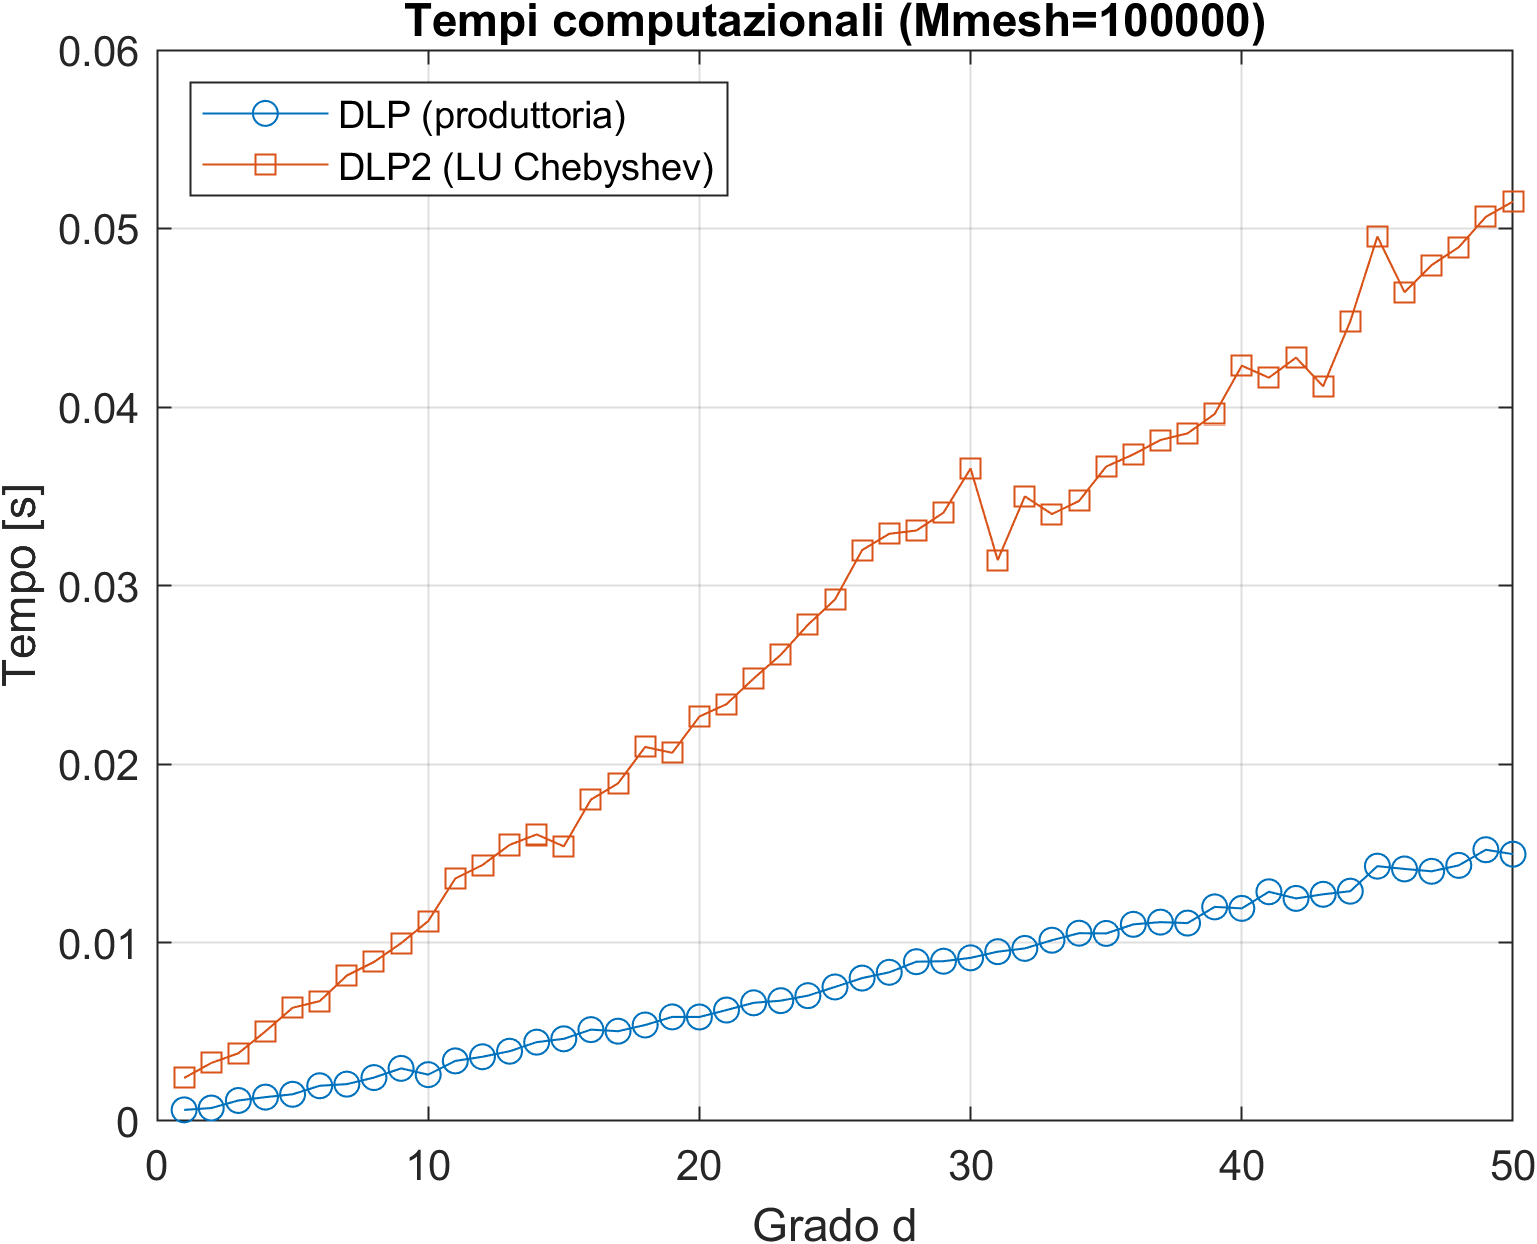
\includegraphics[width=.9\textwidth]{tempi.png}
  \caption{Tempi per l'estrazione dei nodi di Leja: DLP (produttoria) vs DLP2 (LU--Chebyshev).}
\end{figure}

\subsection{Costante di Lebesgue}
La costante di Lebesgue \(\Lambda_d\) misura l'amplificazione dell'errore dei dati nell'interpolazione: un valore moderato implica stabilità numerica. Per nodi ``buoni'' (Chebyshev, Leja) la crescita attesa è \(O(\log d)\) o comunque molto più lenta rispetto ai nodi equispaziati, per i quali la costante cresce rapidamente (quasi esponenziale) causando il fenomeno di Runge.

Nel nostro esperimento \(\Lambda_d\) è stimata come \(\max_{x_k\in \mathcal X}\lambda_d(x_k)\) su una griglia densa \(\mathcal X\) di 5000 (o 10000 nelle repliche finali) punti equispaziati in \([-1,1]\). Questa è un'approssimazione per difetto della vera costante continua, ma sufficiente a evidenziare l'andamento.

Osservazioni dai grafici:
\begin{itemize}
  \item l'andamento cresce lentamente e non mostra esplosioni: conferma che i nodi di Leja selezionati mantengono un buon condizionamento;
  \item le due implementazioni (DLP e DLP2) producono la stessa sequenza di nodi, quindi la curva coincide (differenze numeriche al di sotto di \(10^{-13}\));
  \item per gradi oltre ~40 la crescita si appiattisce leggermente a causa della discretizzazione della griglia e dell'arrotondamento floating point (doppia precisione);
  \item il confronto (non riportato in figura) con nodi equispaziati mostrerebbe valori decisamente maggiori già per gradi medi, giustificando i maggiori errori interpolatori visti nella Sez.~4.3.
\end{itemize}

Dal punto di vista pratico, il valore relativamente contenuto di \(\Lambda_d\) implica che l'errore dell'interpolante sui nodi di Leja è dominato dall'errore di approssimazione della funzione e non dall'amplificazione numerica.

\begin{figure}[htbp!]
  \centering
  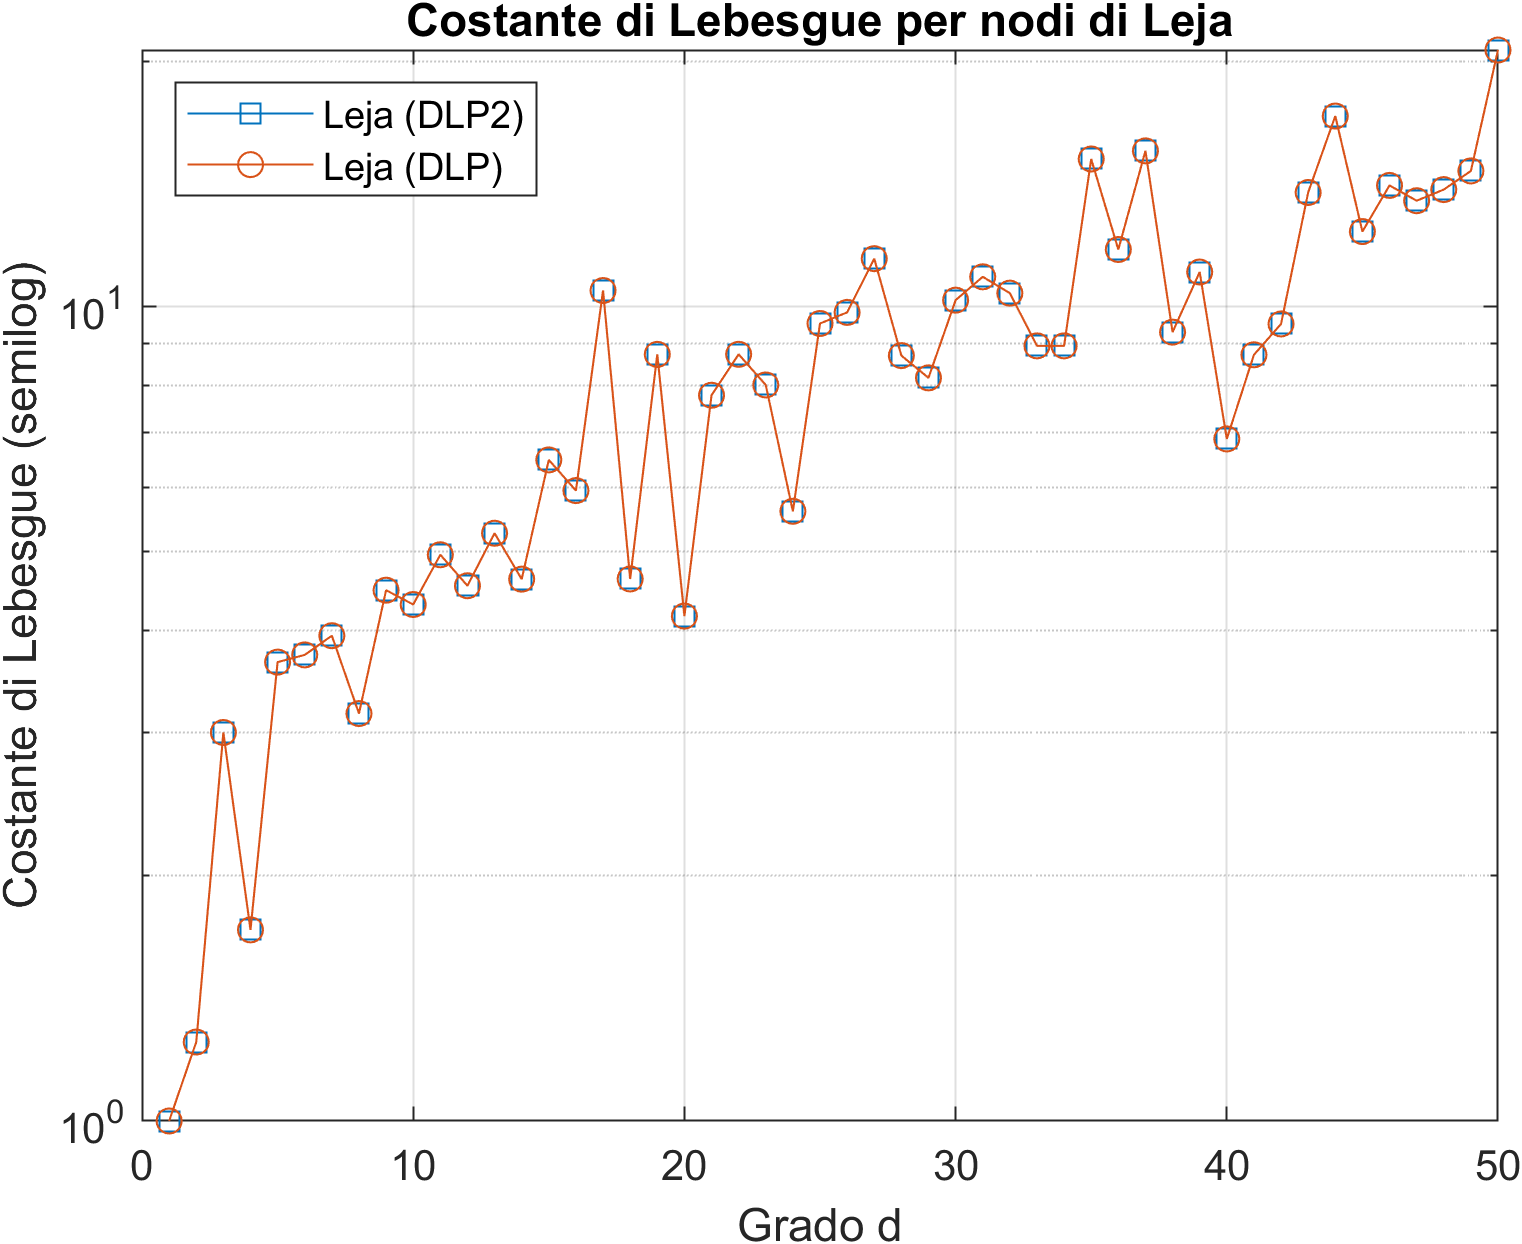
\includegraphics[width=.9\textwidth]{lebesgue.png}
  \caption{Costante di Lebesgue (scala semilog): i due metodi producono gli stessi nodi di Leja.}
\end{figure}

\clearpage
\subsection{Accuratezza dell'interpolante}
Interpolante costruita in base di Chebyshev con i nodi Leja (dall'algoritmo più efficiente) e con nodi equispaziati; confronto dell'errore massimo su griglia densa.
\begin{figure}[htbp!]
  \centering
  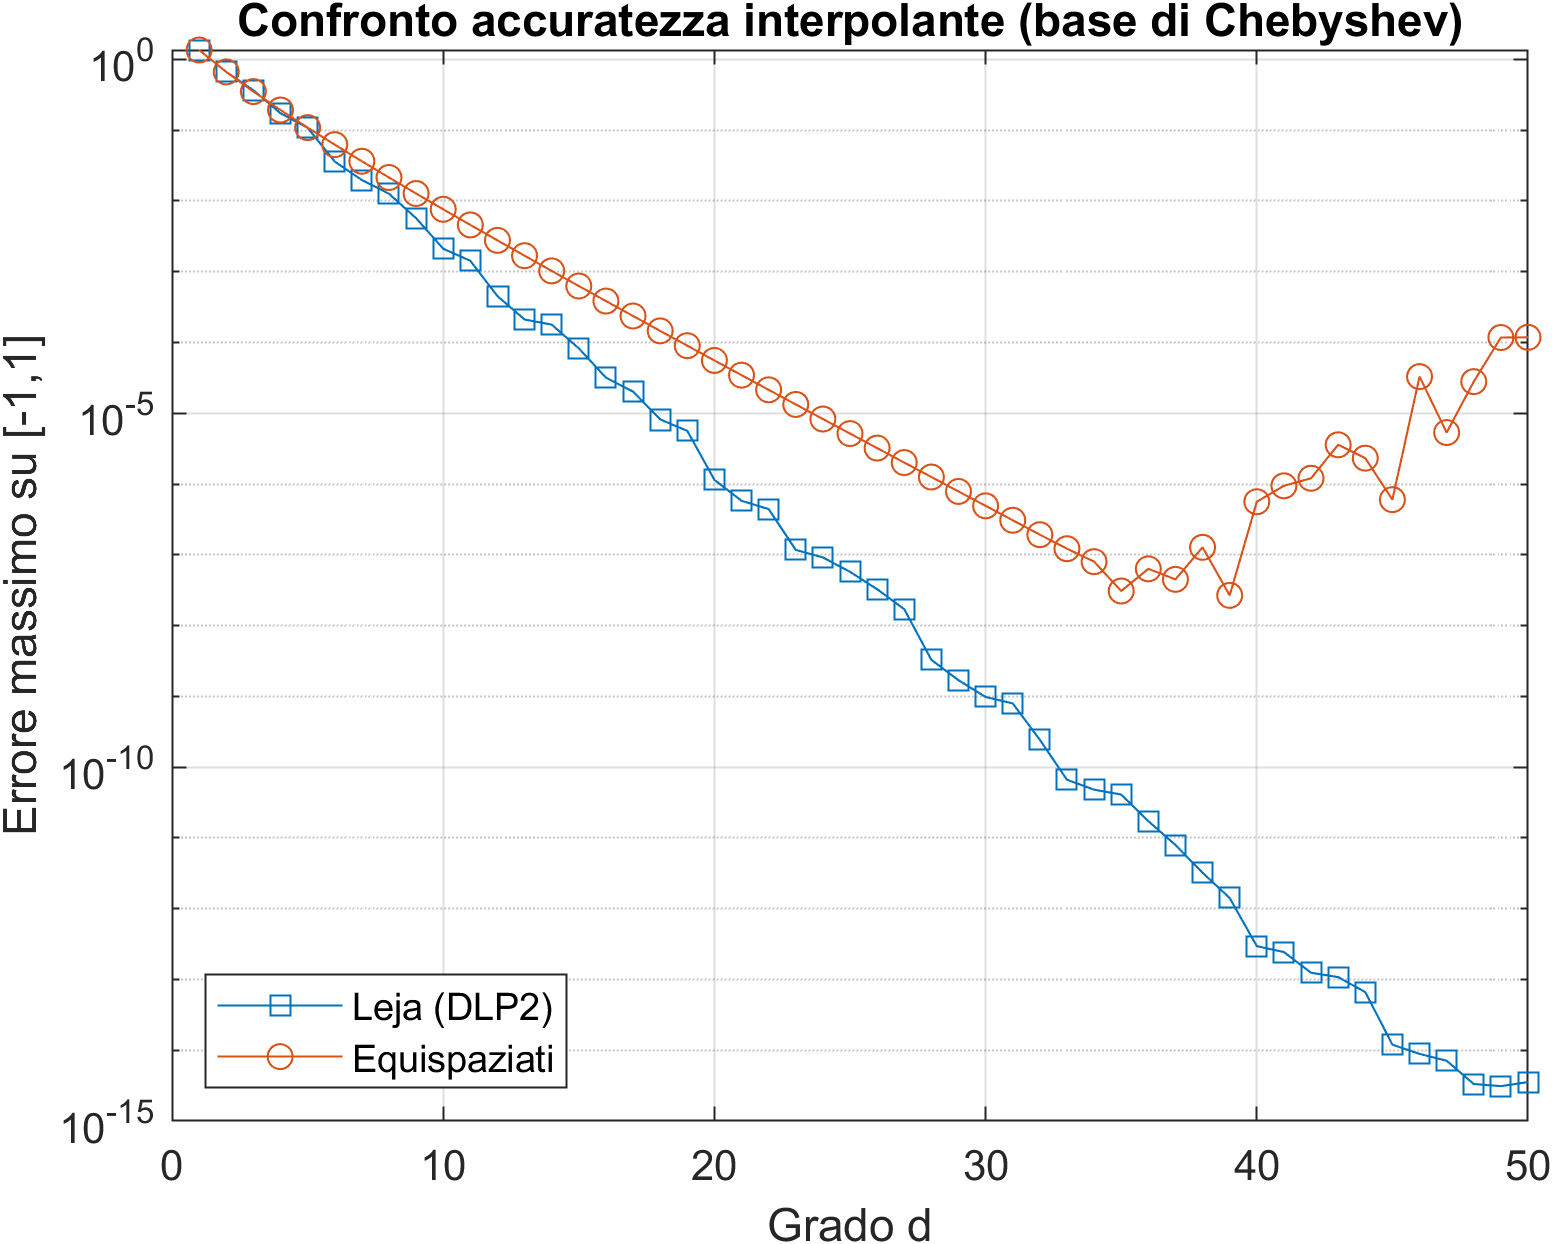
\includegraphics[width=.9\textwidth]{errori.png}
  \caption{Errore massimo dell'interpolante su \([{-}1,1]\): Leja vs equispaziati.}
\end{figure}

% ===================== CONCLUSIONI =====================
\section{Conclusioni}
I risultati mostrano che:
\begin{itemize}
  \item i due algoritmi (\texttt{DLP}, \texttt{DLP2}) estraggono la \emph{stessa} sequenza di nodi di Leja (con \(z_0=x(1)\)), come confermato dall'identità delle costanti di Lebesgue;
  \item l'algoritmo \texttt{DLP} è più veloce per i gradi considerati, mentre \texttt{DLP2} risulta comunque competitivo e più strutturato;
  \item la costante di Lebesgue sui nodi di Leja cresce moderatamente, indicando buona stabilità dell'interpolazione;
  \item l'interpolante su nodi di Leja è nettamente più accurata rispetto a quella su nodi equispaziati, con errori che decrescono fino al limite di macchina.
\end{itemize}

% ===================== APPENDICE (OPZIONALE) =====================
\section*{Appendice: riproducibilità}
Per riprodurre i grafici, eseguire \texttt{main.m} dopo aver posto i sorgenti \texttt{DLP.m}, \texttt{DLP2.m}, \texttt{leb\_con.m} nella stessa cartella. Le figure sono salvate automaticamente in \texttt{doc/img/} (o spostate manualmente prima di compilare).

\end{document}
